\documentclass{standalone}
\usepackage{tikz}
\usetikzlibrary{patterns, positioning}


\begin{document}
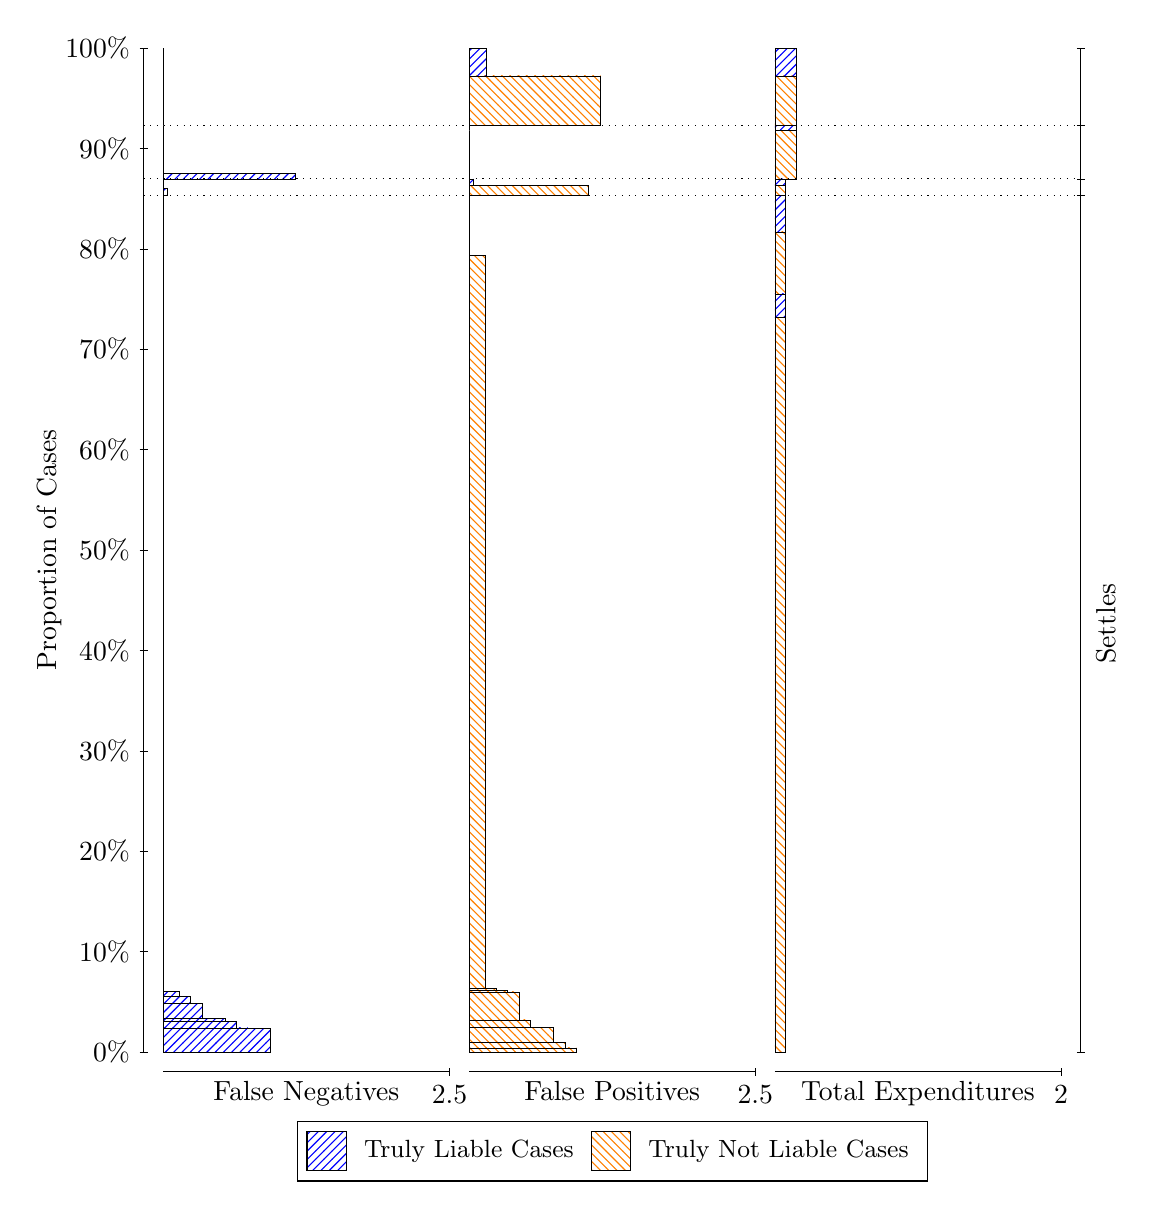
\begin{tikzpicture}
\draw[black, very thin] (1.5,1.75) -- (1.5,14.5);
\node[rotate=90, text=black, anchor=center] at (0.3, 8.125) {Proportion of Cases};
\draw[black, very thin] (1.45,1.75) -- (1.55,1.75);
\node[text=black, anchor=east] at (1.45, 1.75) {0\%};
\draw[black, very thin] (1.45,3.025) -- (1.55,3.025);
\node[text=black, anchor=east] at (1.45, 3.025) {10\%};
\draw[black, very thin] (1.45,4.3) -- (1.55,4.3);
\node[text=black, anchor=east] at (1.45, 4.3) {20\%};
\draw[black, very thin] (1.45,5.575) -- (1.55,5.575);
\node[text=black, anchor=east] at (1.45, 5.575) {30\%};
\draw[black, very thin] (1.45,6.85) -- (1.55,6.85);
\node[text=black, anchor=east] at (1.45, 6.85) {40\%};
\draw[black, very thin] (1.45,8.125) -- (1.55,8.125);
\node[text=black, anchor=east] at (1.45, 8.125) {50\%};
\draw[black, very thin] (1.45,9.4) -- (1.55,9.4);
\node[text=black, anchor=east] at (1.45, 9.4) {60\%};
\draw[black, very thin] (1.45,10.675) -- (1.55,10.675);
\node[text=black, anchor=east] at (1.45, 10.675) {70\%};
\draw[black, very thin] (1.45,11.95) -- (1.55,11.95);
\node[text=black, anchor=east] at (1.45, 11.95) {80\%};
\draw[black, very thin] (1.45,13.225) -- (1.55,13.225);
\node[text=black, anchor=east] at (1.45, 13.225) {90\%};
\draw[black, very thin] (1.45,14.5) -- (1.55,14.5);
\node[text=black, anchor=east] at (1.45, 14.5) {100\%};

\draw[black, very thin] (13.4,1.75) -- (13.4,14.5);
\draw[black, very thin] (13.35,1.75) -- (13.45,1.75);
\node[anchor=west] at (13.35, 1.75) {};
\draw[black, very thin] (13.35,12.629) -- (13.45,12.629);
\node[anchor=west] at (13.35, 12.629) {};
\draw[black, very thin] (13.35,12.838) -- (13.45,12.838);
\node[anchor=west] at (13.35, 12.838) {};
\draw[black, very thin] (13.35,13.518) -- (13.45,13.518);
\node[anchor=west] at (13.35, 13.518) {};
\draw[black, very thin] (13.35,14.5) -- (13.45,14.5);
\node[anchor=west] at (13.35, 14.5) {};

\draw[black, very thin, pattern color=blue, pattern=north east lines] (1.75,1.75) rectangle (3.1125,2.0493);
\draw[black, very thin, pattern color=blue, pattern=north east lines] (1.75,2.0493) rectangle (2.9672,2.0529);
\draw[black, very thin, pattern color=blue, pattern=north east lines] (1.75,2.0529) rectangle (2.8218,2.0566);
\draw[black, very thin, pattern color=blue, pattern=north east lines] (1.75,2.0566) rectangle (2.6765,2.1401);
\draw[black, very thin, pattern color=blue, pattern=north east lines] (1.75,2.1401) rectangle (2.5312,2.1721);
\draw[black, very thin, pattern color=blue, pattern=north east lines] (1.75,2.1721) rectangle (2.2405,2.3651);
\draw[black, very thin, pattern color=blue, pattern=north east lines] (1.75,2.3651) rectangle (2.0952,2.4553);
\draw[black, very thin, pattern color=blue, pattern=north east lines] (1.75,2.4553) rectangle (1.9498,2.5166);
\draw[black, very thin, pattern color=orange, pattern=north west lines] (1.75,2.5166) rectangle (1.75,12.629);
\draw[black, very thin, pattern color=blue, pattern=north east lines] (1.75,12.629) rectangle (1.8045,12.714);
\draw[black, very thin, pattern color=orange, pattern=north west lines] (1.75,12.714) rectangle (1.75,12.838);
\draw[black, very thin, pattern color=blue, pattern=north east lines] (1.75,12.838) rectangle (3.4213,12.906);
\draw[black, very thin, pattern color=orange, pattern=north west lines] (1.75,12.906) rectangle (1.75,13.518);
\draw[black, very thin, pattern color=orange, pattern=north west lines] (1.75,13.518) rectangle (1.75,14.145);
\draw[black, very thin, pattern color=blue, pattern=north east lines] (1.75,14.145) rectangle (1.75,14.5);
\draw[black, very thin, pattern color=orange, pattern=north west lines] (5.6333,1.75) rectangle (6.9958,1.8014);
\draw[black, very thin, pattern color=orange, pattern=north west lines] (5.6333,1.8014) rectangle (6.8505,1.8746);
\draw[black, very thin, pattern color=orange, pattern=north west lines] (5.6333,1.8746) rectangle (6.7052,2.0667);
\draw[black, very thin, pattern color=orange, pattern=north west lines] (5.6333,2.0667) rectangle (6.4145,2.1589);
\draw[black, very thin, pattern color=orange, pattern=north west lines] (5.6333,2.1589) rectangle (6.2692,2.5137);
\draw[black, very thin, pattern color=orange, pattern=north west lines] (5.6333,2.5137) rectangle (6.1238,2.5361);
\draw[black, very thin, pattern color=orange, pattern=north west lines] (5.6333,2.5361) rectangle (5.9785,2.5585);
\draw[black, very thin, pattern color=orange, pattern=north west lines] (5.6333,2.5585) rectangle (5.8332,11.863);
\draw[black, very thin, pattern color=blue, pattern=north east lines] (5.6333,11.863) rectangle (5.6333,12.629);
\draw[black, very thin, pattern color=orange, pattern=north west lines] (5.6333,12.629) rectangle (7.1412,12.753);
\draw[black, very thin, pattern color=blue, pattern=north east lines] (5.6333,12.753) rectangle (5.6878,12.838);
\draw[black, very thin, pattern color=orange, pattern=north west lines] (5.6333,12.838) rectangle (5.6333,13.45);
\draw[black, very thin, pattern color=blue, pattern=north east lines] (5.6333,13.45) rectangle (5.6333,13.518);
\draw[black, very thin, pattern color=orange, pattern=north west lines] (5.6333,13.518) rectangle (7.3047,14.145);
\draw[black, very thin, pattern color=blue, pattern=north east lines] (5.6333,14.145) rectangle (5.8513,14.5);
\draw[black, very thin, pattern color=orange, pattern=north west lines] (9.5167,1.75) rectangle (9.6529,11.076);
\draw[black, very thin, pattern color=blue, pattern=north east lines] (9.5167,11.076) rectangle (9.6529,11.379);
\draw[black, very thin, pattern color=orange, pattern=north west lines] (9.5167,11.379) rectangle (9.6529,12.165);
\draw[black, very thin, pattern color=blue, pattern=north east lines] (9.5167,12.165) rectangle (9.6529,12.629);
\draw[black, very thin, pattern color=orange, pattern=north west lines] (9.5167,12.629) rectangle (9.6529,12.753);
\draw[black, very thin, pattern color=blue, pattern=north east lines] (9.5167,12.753) rectangle (9.6529,12.838);
\draw[black, very thin, pattern color=orange, pattern=north west lines] (9.5167,12.838) rectangle (9.7892,13.45);
\draw[black, very thin, pattern color=blue, pattern=north east lines] (9.5167,13.45) rectangle (9.7892,13.518);
\draw[black, very thin, pattern color=orange, pattern=north west lines] (9.5167,13.518) rectangle (9.7892,14.145);
\draw[black, very thin, pattern color=blue, pattern=north east lines] (9.5167,14.145) rectangle (9.7892,14.5);
\draw[black, dotted] (1.5,12.629) -- (13.4,12.629);
\draw[black, dotted] (1.5,12.838) -- (13.4,12.838);
\draw[black, dotted] (1.5,13.518) -- (13.4,13.518);
\draw[black, very thin] (1.75,1.5) -- (5.3833,1.5);
\node[text=black, anchor=north] at (3.5667, 1.5) {False Negatives};
\draw[black, very thin] (5.3833,1.45) -- (5.3833,1.55);
\node[text=black, anchor=north] at (5.3833, 1.45) {2.5};

\draw[black, very thin] (5.6333,1.5) -- (9.2667,1.5);
\node[text=black, anchor=north] at (7.45, 1.5) {False Positives};
\draw[black, very thin] (9.2667,1.45) -- (9.2667,1.55);
\node[text=black, anchor=north] at (9.2667, 1.45) {2.5};

\draw[black, very thin] (9.5167,1.5) -- (13.15,1.5);
\node[text=black, anchor=north] at (11.333, 1.5) {Total Expenditures};
\draw[black, very thin] (13.15,1.45) -- (13.15,1.55);
\node[text=black, anchor=north] at (13.15, 1.45) {2};

\node[text=black, centered, rotate=90] at (13.72, 7.1896) {Settles};




\draw (7.449999999999999,1.5) node[draw=none] (baseCoordinate) {};
\begin{scope}[align=center]
        \matrix[scale=0.5, draw=black, below=0.5cm of baseCoordinate, nodes={draw}, column sep=0.1cm]{
            \node[rectangle, draw, minimum width=0.5cm, minimum height=0.5cm, pattern color=blue, pattern=north east lines] {}; &
            \node[draw=none, font=\small, text=black] (B) {Truly Liable Cases}; &
            \node[rectangle, draw, minimum width=0.5cm, minimum height=0.5cm, pattern color=orange, pattern=north west lines] {}; &
            \node[draw=none, font=\small, text=black] (B) {Truly Not Liable Cases}; \\
            };
\end{scope}

\end{tikzpicture}
\end{document}